\chapter{Learning Methods}

This chapter provides a framing of the visual field progression prediction tasks introduced before as learning problems, and introduces the learning algorithm architectures to be evaluated against the available data set. 

\section{The Learning Task}

\subsection{Formulation and Normalization}

Given the information in the Rotterdam dataset, we can write each patient visit as one feature vector as follows:

\begin{equation}
v^{(i)} = \begin{bmatrix}
\textrm{VF}^{(i)}_1 & 
\textrm{VF}^{(i)}_2 & 
\cdots & 
\textrm{VF}^{(i)}_{54} & 
\textrm{MD}^{(i)} & 
\textrm{IOP}^{(i)} & 
t^{(i)}
\end{bmatrix}
\in \mathbb{R}^{57}
\end{equation}

where $t^{(n)}$ is the time of the visit, and $\textrm{VF}^{(i)}_j$ is the \ac{DLS} for the $j$-th point in the visual field. By convention of the visual field analysis tools developed by Marin-Franch et al. \cite{Marin-Franch2013}, all fields of the left (OS) eye are flipped horizontally (unmodified vertically) to match with the coordinates of the right eye, and then each visual field location is index from left to right, then top to bottom, in the same way as the reading direction in English. Each of the vector component is normalized in the range shown in \cref{tab:norm}.

\begin{table}[h]
\centering
\caption{Feature range normalization with appropriate physiological ranges}
\begin{tabular}{@{}lrrrc@{}}
\toprule
 & \multicolumn{3}{c}{Normalization Range} & \\
\cmidrule{2-4}
Feature & Lower (0) & Upper (1) & Unit & Comments \\ 
\midrule
VF & 0 & 40 & dB &  \\
MD & 0 & 40 & dB & Negative sign preserved \\
IOP & 0 & 20 & mmHg &  \\
Age ($t$) & 50 & 80 & years &  \\ 
\bottomrule
\end{tabular}
\label{tab:norm}
\end{table}

For three input fields, we can concatenate the three visits and write the entire input vector as: 

\begin{equation}
x^{(n)} = \begin{bmatrix}
v^{(i)} & v^{(i+1)} & v^{(i+1)}
\end{bmatrix}
\in \mathbb{R}^{171}
\end{equation}

\subsection{Learning Dataset Generation}

The entire dataset can be put into matrix form, where the input is:

\begin{equation}
\mathbf{X} = \begin{bmatrix}
x^{(1)} \\
x^{(2)} \\
\vdots \\
x^{(N)} \\
\end{bmatrix}
\in \mathbb{R}^{N\times 161}
\end{equation}

and the output field prediction is simply the \ac{DLS} at each location:

\begin{equation}
\mathbf{Y} = \begin{bmatrix}
Y^{(1)} \\
Y^{(2)} \\
\vdots \\
Y^{(N)} \\
\end{bmatrix}
= \begin{bmatrix}
\textrm{VF}_1^{(1)} & \textrm{VF}_2^{(1)} & \cdots & \textrm{VF}_{54}^{(1)} \\
\textrm{VF}_1^{(2)} & \textrm{VF}_2^{(2)} & \cdots & \textrm{VF}_{54}^{(2)} \\
& \vdots & & \\
\textrm{VF}_1^{(N)} & \textrm{VF}_2^{(N)} & \cdots & \textrm{VF}_{54}^{(N)}
\end{bmatrix}
\in \mathbb{R}^{N\times 54}
\end{equation}

Since it is fairly standard---and also the case in the Rotterdam dataset as shown before---that glaucoma patients are followed up on an interval of 6 months, the training examples are generated such that

\begin{equation} \label{eq:train-criterion-1}
\Delta t = 183~\textrm{days} \approx (t_{v^{(i+1)}} - t_{v^{(i)}}) \approx (t_{v^{(i+2)}} - t_{v^{(i+1)}})
\end{equation}

and the output field is $K$ fields (approximately $0.5K$ years) after the last input field:

\begin{equation} \label{eq:train-criterion-2}
t_{v^{(Y)}} - t_{v^{(i+1)}} \approx 183K~\textrm{days}
\end{equation}

Learning sets in the Rotterdam dataset that satisfy \cref{eq:train-criterion-1,,eq:train-criterion-2} for all $K\in[1, 10]$ are generated.

\subsection{Error Definition}

The \ac{MAE} error for the whole field is defined as:

\begin{equation}
L(\hat{y}, y) = \textrm{MAE}_{\vf} \triangleq 
\frac{1}{54N} \sum_{n=1}^N \sum_{j=1}^{54} \left|  \widehat{\vf}_j^{(n)} - {\vf}_j^{(n)}  \right|
\end{equation}

The \ac{MAE} error for \ac{MD} is defined as:

\begin{equation} \label{eq:mae-md}
%\textrm{MAE}_{\md} \triangleq
\frac{1}{N} \sum_{n=1}^N \left|  \widehat{\md}^{(n)} - {\md}^{(n)}  \right|
\end{equation}

The calculation of \ac{MD} was introduced as \cref{eq:md}, which requires 1) age-adjusted baseline \ac{DLS} values and 2) variance at each location of the field (i.e. weights when averaging the deviation values). Since the target \ac{MD} values in the Rotterdam database are provided presumably from \ac{HFA}'s database that are not publicly available, one can modify \cref{eq:mae-md} by substituting in \cref{eq:md}:

\begin{align}
\textrm{MAE}_{\md} &=
\frac{1}{N} \sum_{n=1}^N \left| 
\sum_{j=1}^{54} w_j \left( \widehat{\vf}_j^{(n)} - N_j \right) - 
\sum_{j=1}^{54} w_j \left( {\vf}_j^{(n)} - N_j \right)  \right| \\
&=
\frac{1}{N} \sum_{n=1}^N \left| 
\sum_{j=1}^{54} w_j \left( \widehat{\vf}_j^{(n)} - \vf_j^{(n)} \right) \right|
\end{align}

where $N_j$ is the age-adjusted population normal value at the $j$-th visual field point, and 

\begin{equation}
w_j=\frac{ \frac{1}{\sigma_{j}^2} }{
	\sum\limits_{i=1}^{n} 
	\frac{1}{\sigma_{i}^2} 
}
\end{equation}

. This expression is only dependent upon the weights used in calculating \ac{MD}, since the age-adjusted baseline cancels out. The weights are available from Heijl et al. \cite{Heijl1987} or Marin-Franch et al. \cite{Marin-Franch2013}

\subsection{Evaluation Procedure}

$70\%$ of the data is used for training, $15\%$ is used for validation and used to fine tune the hyper-parameters of the model. Then, the hyper-parameters are set and 5- or 10-fold cross validation is performed to report model performance. 

\section{Models}

This section describes a range of simple to complex learning models that are proposed for evaluation for the learning task. Simpler models might be more robust to noise in the visual field dataset and generalize better for the limited data available, while a complex model might extract more powerful visual field and patient features from the data at the peril of over-fitting. 

\subsection{Ridge Regression}

Ridge regression is a $L_2$-regularized linear regression\footnotemark that aims to minimize the combination of the sum squared cost and the $L_2$ norm of the weight parameters. By weighting on the model parameters, one hopes to yield a simpler model that is fit less toward specific trends in the training set and generalizes better. The model prediction is: 

\footnotetext{In this document the term ``linear regression'' is intentionally avoided to avoid confusion with the simple linear extrapolation method by extrapolating each variable with a linear fit over time, which is often called the \ac{OLSLR} method.}

\begin{equation}
\hat{\mathbf{Y}} = \mathbf{X}_1\mathbf{W}
\end{equation}

where $\mathbf{X}_1\triangleq\begin{bmatrix}\mathbf{1} & \mathbf{X} \end{bmatrix}$ includes the bias feature. The objective is to minimize the regularized sums squared cost:

\begin{equation}
\mathbf{W} \leftarrow \arg \min_{\mathbf{W}} ||\hat{\mathbf{Y}} - \mathbf{Y}||^2_2 + \lambda ||\mathbf{W}||^2_2
\end{equation}

This has the closed form solution, which is directly implemented:

\begin{equation}
\mathbf{W} = \left(
\mathbf{X}_1^T \mathbf{X}_1 + \lambda I
\right)^{-1}
\mathbf{X}_1^T \mathbf{Y}
\end{equation}

\subsection{Huber Regression}

The Huber linear regressor uses a cost metric that is more robust to outliers, with the following definition:

\begin{equation}
L(\hat{y}_j, y_j) = \left\{\begin{array}{lr}
\frac{1}{2}(\hat{y}_j - y_j)^2, & |\hat{y}_j - y_j| \leq \delta\\
\delta|\hat{y}_j - y_j| - \frac{1}{2} \delta^2, & |\hat{y}_j - y_j| > \delta\\
\end{array}
\right.
\end{equation}

Intuitively, for points close to the target, a squared cost is used, while for points further away than a threshold (e.g. outliers), a linear cost is used. Therefore it is also known as a robust regressor. One may hope that it may be better at rejecting noise from visual field recordings. 

One Huber regressor is needed for each output dimension, so essentially 54 regressors are fit with the same input. Implementation wise, this is done by chaining \verb|HuberRegressor| into \verb|MultiOutputRegressor| using the Scikit-learn library. \cite{scikit-learn} There is no closed-form solution for Huber regression so an iterative solution is found. 

\subsection{Multi-Layer Perceptron}

The \ac{MLP} neural network model takes the 171 features as input and outputs 54 \ac{DLS} values. Considering the high dimensionality of the output, a standard three-layer (two hidden layers) network is investigated with number of neural units being the hyperparameter. $L_2$ regularization is applied to all weights. ReLU is used as the activation function at all layers except the output layer. The model is implemented in Tensorflow. \cite{tensorflow} The whole field \ac{MAE} loss is used as the objective function. The weights are optimized iteratively with the Adam Optimizer using batch size of 32.

\subsection{Convolutional Neural Network}

\ac{CNN} is a type of neural network architecture that, thanks to the tremendous improvement in computational power recently, has shown tremendous performance in automatically learning to extract image features instead of requiring hand-crated features detection algorithms. Each visual field can be seen as an $8\times9$ image. This relatively low dimensionality, compared to the inputs to typical image recognitions tasks in which \acp{CNN} are applied, may leave limited room of improvement in the performance of \ac{CNN} over a simpler flat architecture such as \iac{MLP}. However, spatial patterns in the visual field are have been known to important to glaucoma diagnosis and progression, and \ac{CNN} is an architecture that is known to be able to extract such spatial information. 

\begin{figure}[p]
	\centering
	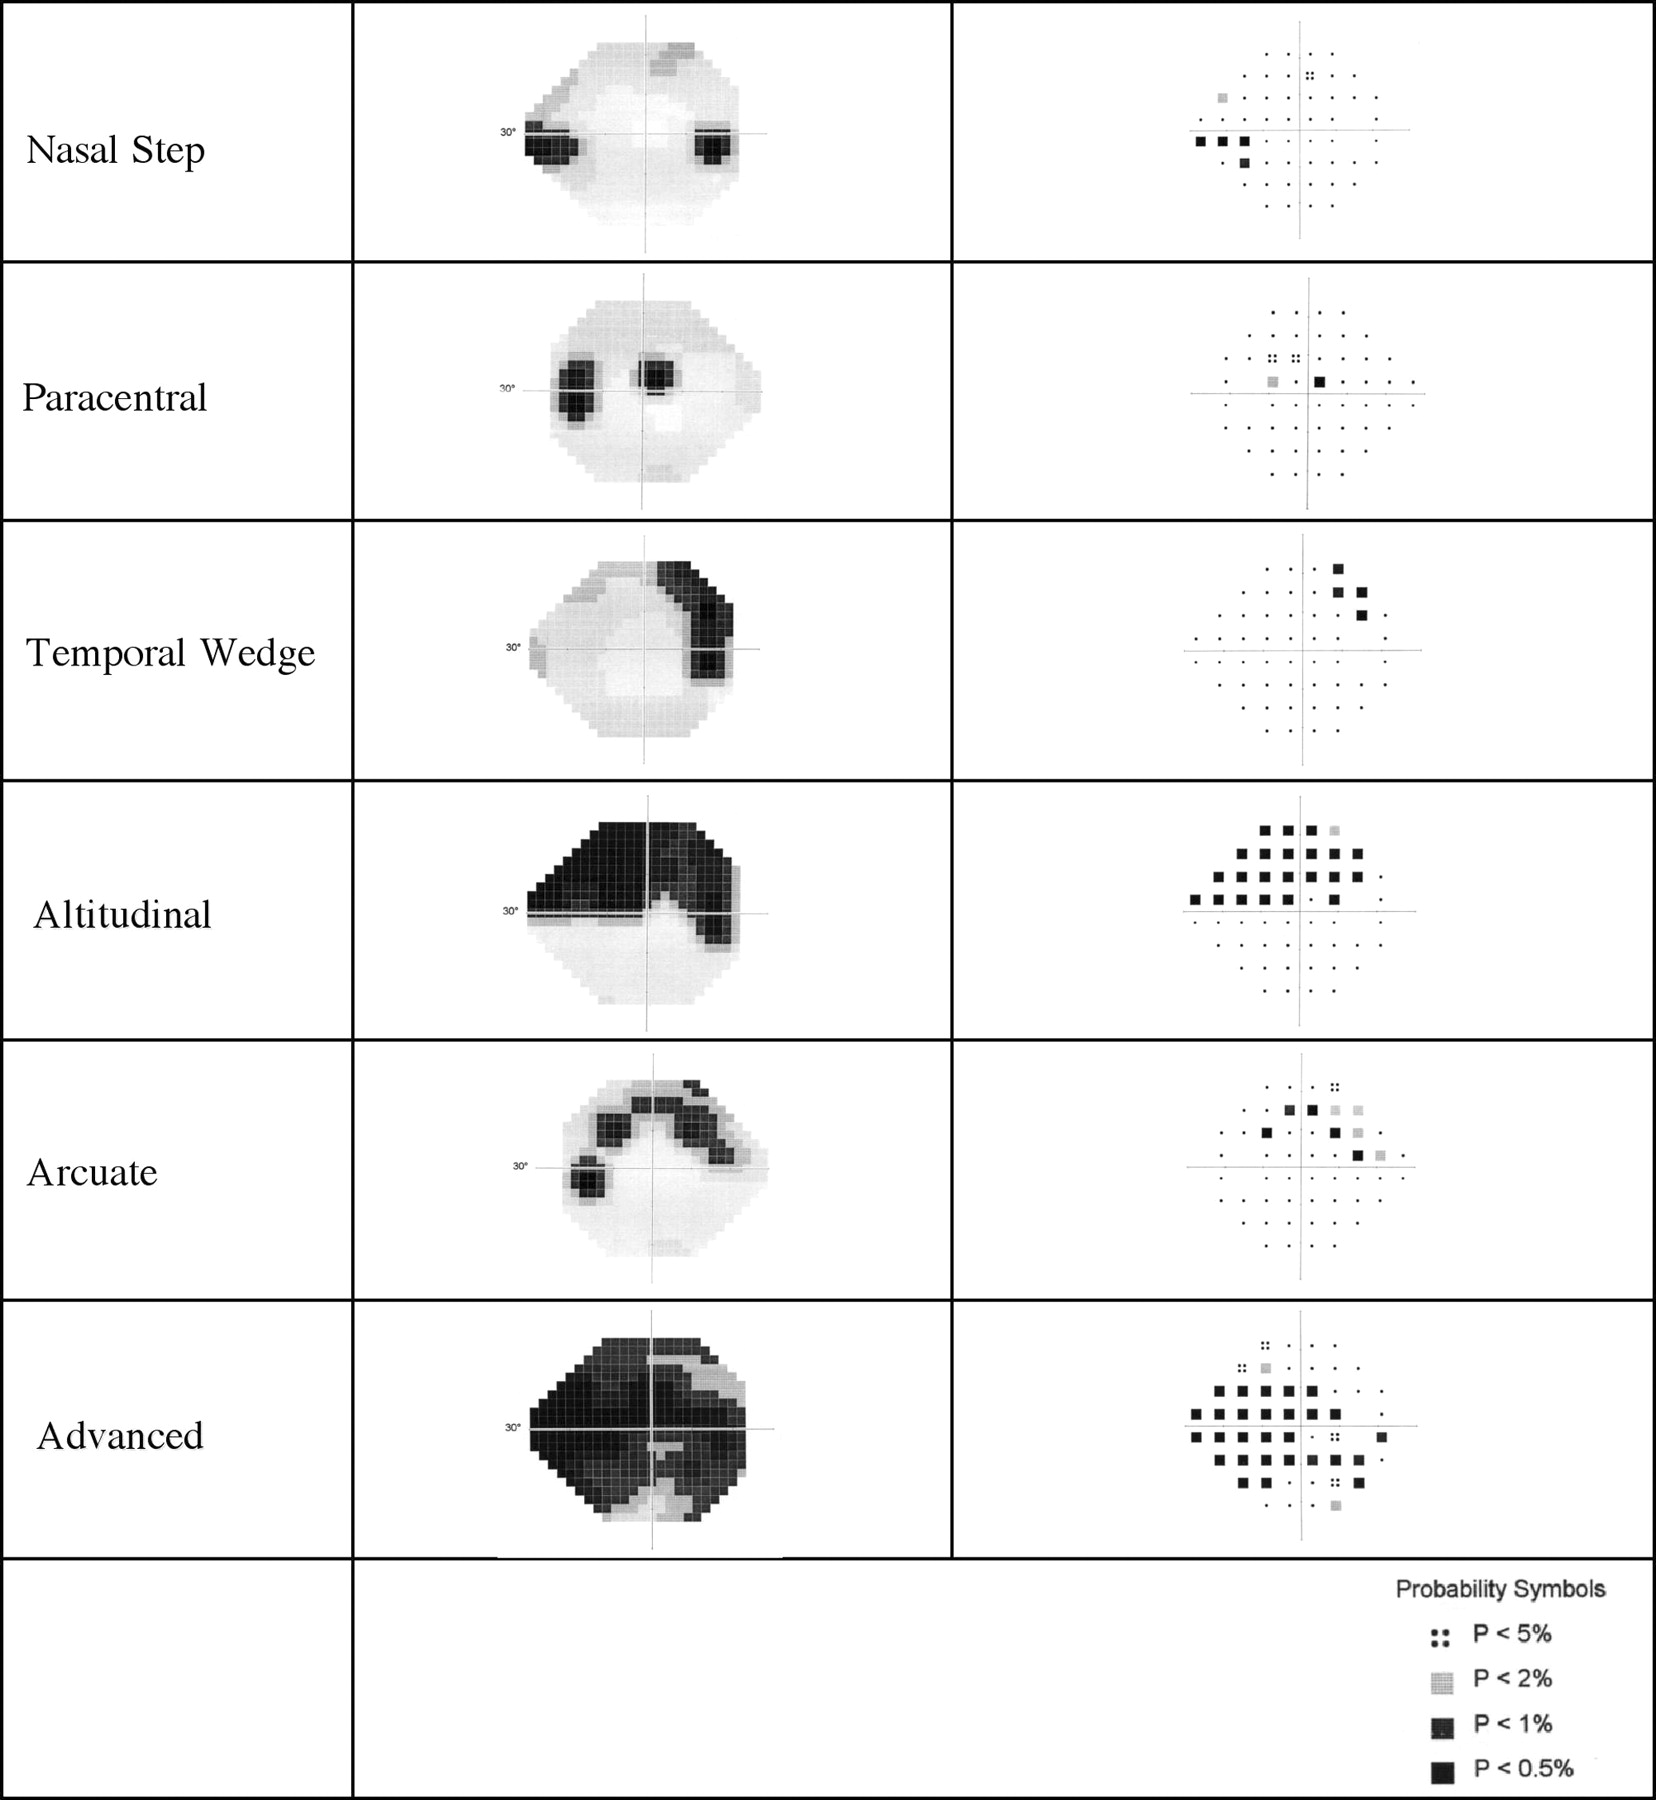
\includegraphics[width=\textwidth]{sample2004pattern}
	\caption[Examples of typical patterns of glaucomatous visual field loss]{Examples of typical patterns of glaucomatous visual field loss that are known to be physiologically and clinically important for diagnosis and prediction. Such evidence is the motivation behind employing a \ac{CNN} achitecture that is likely to preserve and extract useful spatial information in the visual field. (Figure from Sample et al. \cite{Sample2004})}
\end{figure}

A typical \ac{CNN} architecture is implemented. Specifically, this \ac{CNN} consists of:

\begin{enumerate}
\item Input layer: Input is three visual field ``images'' stacked ($8\times9\times3$). Locations outside the 24-2 examination area are replaced with zeros. 
\item First convolutional layer with $3\times3$ kernel, stride length $1$. Output is passed through ReLU activation and batch normalization. 
\item Max pool layer with pool size and stride length of $2$. 
\item Second convolutional layer with $3\times3$ kernel, stride length $1$. Output is passed through ReLU activation and batch normalization, then flattened. 
\item Additional features (i.e. MD, IOP, and Age) are concatenated to the vector. 
\item First fully connected hidden layer. Output is passed through ReLU activation and a dropout layer. 
\item Second fully connected hidden layer. 
\item Output layer. ($d=54$)
\end{enumerate}

The modeled is trained using Adam Optimizer to minimize the $L_2$ regularized \ac{MAE} loss, and implemented with Tensorflow. \cite{tensorflow} The number of channels in the \ac{CNN}, neural units in the fully-connected layer, and regularization are fine-tuned as hyperparameters. 

\subsection{Deep CNN+LSTM Network}

The final proposed framework involves adding the \ac{LSTM} network to the \ac{CNN} network. The \ac{LSTM} module is a type of \ac{RNN}. Its recurrent nature allows modeling of sequential data; in the case of the current prediction task, it is used to model the sequential visual field inputs at different time points. 

The \ac{LSTM} network also has the benefit of only needing one network to predict multiple outputs in the future due to its recurrent nature. Because of this, the training dataset used to train this network is slightly different from networks above. When training this network, it is necessary to generate a sequence of all fields $i=0, 1, 2, (2+1), (2+2), \dots, (2+K)$ where $K$ is the maximum number of fields in the future that is desired to be predicted. At test time, the model takes fields $i=0, 1, 2$ as input, and outputs all field predictions at $i=(2+1), (2+2), \dots, (2+K)$. $K=5$ and $K=10$ are tested, where $K=5$ is expected to include more training examples. 

The detailed procedure of this network is shown as \cref{algo:CNNLSTM} in \cref{chapter:code}. The network is implemented using the PyTorch framework. \cite{paszke2017automatic} 


